\documentclass[12pt,reqno]{amsart}

\usepackage[tmargin=35mm,bmargin=35mm,lmargin=35mm,rmargin=35mm]{geometry}
\usepackage{rotate,graphicx,url}
\usepackage[brazil]{babel}
\usepackage[utf8]{inputenc}
\usepackage[alf]{abntex2cite}
\usepackage{amsaddr}
\usepackage{float}
\usepackage{booktabs}
\usepackage{multirow}
\usepackage{microtype}
\usepackage{amsmath,amssymb}
\usepackage{fancyhdr}

% Número da página no rodapé (inclusive na primeira página)
\pagestyle{fancy}
\fancyhf{}
\fancyhead[C]{\small\scshape Aplicação do Algoritmo Double K-Means na Base de Dados Spambase}
\fancyfoot[C]{\small \thepage}
\renewcommand{\headrulewidth}{0pt}
\fancypagestyle{plain}{\fancyhf{}\fancyfoot[C]{\small \thepage}}
\fancypagestyle{firstpage}{\fancyhf{}\fancyfoot[C]{\small \thepage}}
\setlength{\headheight}{15pt}
\setlength{\emergencystretch}{2em} % evita linhas passando da margem

\begin{document}

\title{Aplicação do Algoritmo Double K-Means na Base de Dados Spambase}

\author{Bruno Henrique Santos de Almeida \\
Pamella Vitoria Gomes Farias \\
Rozyelayny Nascimento} 

\address{Universidade Federal de Pernambuco \\
Programa de Pós Graduação em Ciência da Computação}

\keywords{Agrupamento, K-Means, Spambase, Spam, Double K-Means}

\begin{abstract}
O presente artigo aplica o método de agrupamento Double K-Means na base de dados Spambase, com o objetivo de identificar padrões e características que diferenciam e-mails legítimos de mensagens de spam. 

\end{abstract}

\maketitle 

\section{Introdução}

\section{Algoritmo Double K-Means}


\section{Base de Dados}

A base \emph{Spambase}, do repositório UCI (\url{https://archive.ics.uci.edu/dataset/94/spambase}),
foi criada em 1999 nos laboratórios da Hewlett-Packard (HP Labs) a partir de e-mails reais.
Os spams vieram de denúncias de usuários e os e-mails legítimos vieram de mensagens pessoais
e de trabalho dos funcionários. Ela tem \textbf{4601 e-mails}, cada um descrito por
\textbf{57 atributos numéricos contínuos} e por uma classe binária, \texttt{is\_spam}. Não há
valores ausentes.

\subsection*{Atributos}
Os atributos são frequências calculadas sobre o texto de cada e-mail e formam três grupos
(Tabela~\ref{tab:atributos}).

\begin{table}[H]
\centering
\caption{Grupos de atributos da Spambase.}
\label{tab:atributos}
\small
\begin{tabular}{p{0.30\textwidth}cp{0.48\textwidth}}
\toprule
Grupo & Qtd. & Descrição \\
\midrule
\texttt{word\_freq\_}\emph{PALAVRA} & 48 & Percentual (0--100) das palavras do e-mail iguais a
\emph{PALAVRA} (ex.: \texttt{make}, \texttt{free}, \texttt{money}, \texttt{hp}, \texttt{george}, \texttt{edu}). \\
\texttt{char\_freq\_}\emph{CARACTERE} & 6 & Percentual (0--100) dos caracteres iguais a
\texttt{;} \texttt{(} \texttt{[} \texttt{!} \texttt{\$} \texttt{\#}. \\
\texttt{capital\_run\_length\_*} & 3 & Média (\texttt{average}), maior (\texttt{longest}) e
soma (\texttt{total}) dos comprimentos das sequências contínuas de letras maiúsculas. \\
\midrule
\texttt{is\_spam} (classe) & 1 & 1 = spam, 0 = não-spam. \\
\bottomrule
\end{tabular}
\end{table}

\subsection*{Distribuição das classes}
A base é moderadamente desbalanceada: são \textbf{1813 spams (39,4\%)} e \textbf{2788
e-mails legítimos (60,6\%)}. Por isso todas as divisões em treino e teste da Questão~2 usam
amostragem estratificada, que preserva essas proporções.

\subsection*{Características relevantes}
\begin{itemize}
\item \textbf{Esparsidade:} 77,4\% dos valores da matriz de dados são zero, já que cada e-mail usa
  poucas das 48 palavras monitoradas. Das 57 variáveis, 46 têm mais de 70\% de zeros e 19 têm
  mais de 90\%.
\item \textbf{Escalas muito diferentes:} as frequências ficam entre 0 e 100 (na maioria das
  vezes abaixo de 1), enquanto os atributos de maiúsculas chegam a milhares. Por exemplo,
  \texttt{capital\_run\_length\_total} tem mediana 95 e máximo 15\,841.
\item \textbf{Forte assimetria:} as distribuições têm cauda longa à direita (assimetria mediana
  de 9,7 entre as variáveis, chegando a 31) e muitos valores discrepantes.
\item \textbf{Registros repetidos:} há 391 linhas duplicadas, mantidas como na base original.
\end{itemize}

A Tabela~\ref{tab:medias} mostra que alguns atributos separam bem as classes. Palavras e
símbolos comerciais (\texttt{remove}, \texttt{free}, \texttt{your}, \texttt{!}, \texttt{\$}) e o
uso de maiúsculas são muito mais frequentes nos spams. Já \texttt{hp}, \texttt{george} e
\texttt{edu} aparecem quase só nos e-mails legítimos, pois refletem o ambiente da HP Labs
(George Forman é um dos autores da base). Essa origem explica o pequeno grupo de e-mails
internos encontrado pelo double k-means na Questão~1.

\begin{table}[H]
\centering
\caption{Média de atributos selecionados por classe.}
\label{tab:medias}
\small
\begin{tabular}{lrr}
\toprule
Atributo & Não-spam & Spam \\
\midrule
\texttt{word\_freq\_remove} & 0,009 & 0,275 \\
\texttt{word\_freq\_free} & 0,074 & 0,518 \\
\texttt{word\_freq\_your} & 0,439 & 1,380 \\
\texttt{char\_freq\_!} & 0,110 & 0,514 \\
\texttt{char\_freq\_\$} & 0,012 & 0,174 \\
\texttt{capital\_run\_length\_total} & 161,47 & 470,62 \\
\midrule
\texttt{word\_freq\_hp} & 0,895 & 0,017 \\
\texttt{word\_freq\_george} & 1,265 & 0,002 \\
\texttt{word\_freq\_edu} & 0,287 & 0,015 \\
\bottomrule
\end{tabular}
\end{table}

\subsection*{Pré-processamento}
Por causa das escalas tão diferentes, todos os atributos foram padronizados (\emph{z-score}:
média zero e desvio-padrão um). Na Questão~1, que é não supervisionada, a padronização usa a
base inteira. Na Questão~2, a média e o desvio são estimados apenas no conjunto de treinamento
de cada fold e depois aplicados ao teste, para não vazar informação do teste para o modelo.
Nenhum atributo ou registro foi removido.


\section{Questões}


\subsection{Questão 1:}

\subsubsection*{Organização do experimento}
Os 57 atributos foram padronizados (\emph{z-score}) sobre toda a base, pois têm escalas muito
diferentes (os atributos \texttt{capital\_run\_length\_*} chegam a milhares, enquanto as
frequências de palavras ficam entre 0 e 100). O double k-means minimiza
\[
W(G,U,V)=\sum_{k=1}^{K}\sum_{h=1}^{H}\sum_{i=1}^{N}\sum_{j=1}^{P}u_{ik}\,v_{jh}\,(x_{ij}-g_{kh})^2
\]
alternando três passos: (1) cálculo dos protótipos ótimos
$g_{kh}=\frac{1}{n_k n_h}\sum_{i\in P_k}\sum_{j\in Q_h}x_{ij}$, com $U$ e $V$ fixos;
(2) realocação dos objetos, com $G$ e $V$ fixos; e (3) realocação das variáveis, com $G$ e $U$
fixos. Os passos se repetem enquanto houver transferência de objetos ou de variáveis. Se um grupo
fica vazio, ele recebe o elemento mais distante do protótipo do próprio grupo.

Para cada $K\in\{2,3,4\}$ e $H\in\{1,\dots,K\}$ (9 pares), o algoritmo foi executado
\textbf{100 vezes} a partir de partições iniciais aleatórias, e foi mantida a execução de menor
$W$. As 100 execuções de cada par rodaram em paralelo em uma GPU NVIDIA A100 (PyTorch), cerca de
1~s por par. Todas convergiram. Para a melhor solução de cada par calculou-se a silhueta da
partição dos objetos (distância euclidiana nos dados padronizados).

\subsubsection*{Silhueta e escolha de $K^*$}
A Tabela~\ref{tab:q1} e a Figura~\ref{fig:q1sil} mostram os resultados. A silhueta é máxima no
par $(K,H)=(2,2)$, com valor $0{,}660$, bem acima dos demais (todos $\le 0{,}30$). Portanto,
\[
K^*=\arg\max_{(K,H)} \mathrm{Sil}(K,H)=2 .
\]

\begin{table}[H]
\centering
\caption{Melhor solução (menor $W$ em 100 execuções) de cada par $(K,H)$.}
\label{tab:q1}
\small
\begin{tabular}{ccrrcc}
\toprule
$K$ & $H$ & $W$ (melhor) & Iterações & Tamanho dos grupos & Silhueta \\
\midrule
2 & 1 & 256\,513,75 & 11 & [3583, 1018] & 0,2961 \\
2 & 2 & 244\,486,70 & 40 & [4567, 34] & \textbf{0,6596} \\
3 & 1 & 254\,414,01 & 40 & [1187, 3382, 32] & 0,2515 \\
3 & 2 & 239\,373,66 & 60 & [34, 3470, 1097] & 0,2454 \\
3 & 3 & 234\,585,87 & 34 & [34, 3373, 1194] & 0,1409 \\
4 & 1 & 253\,278,68 & 38 & [2242, 22, 697, 1640] & 0,0484 \\
4 & 2 & 233\,358,70 & 35 & [3275, 1049, 253, 24] & 0,2428 \\
4 & 3 & 228\,516,44 & 45 & [24, 3256, 1080, 241] & 0,1620 \\
4 & 4 & 227\,086,08 & 49 & [26, 1039, 3249, 287] & 0,1697 \\
\bottomrule
\end{tabular}
\end{table}

\begin{figure}[H]
\centering
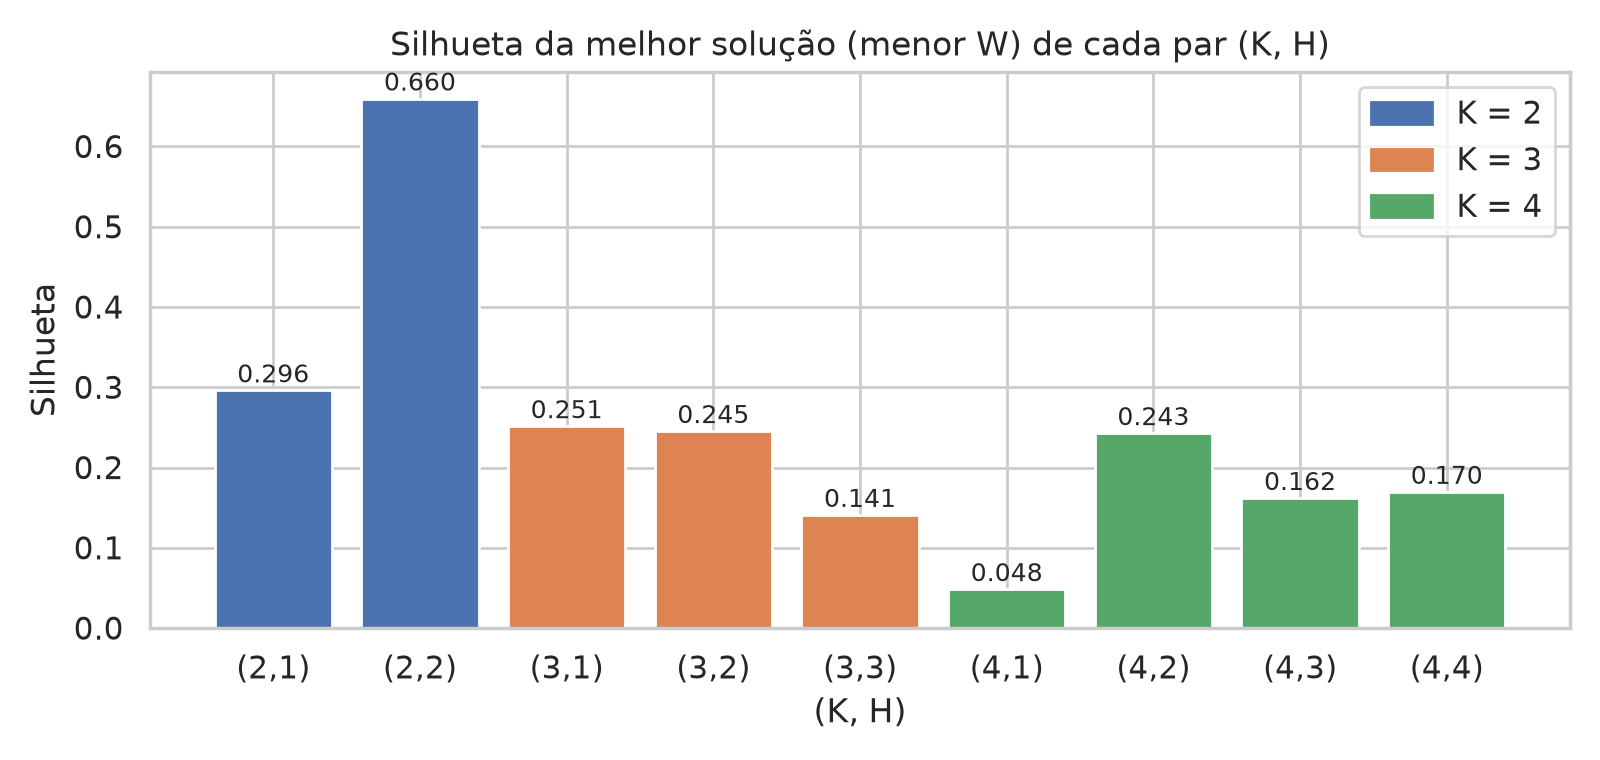
\includegraphics[width=0.85\textwidth]{resultados_versao_final/q1_silhueta.png}
\caption{Silhueta $\times$ $(K,H)$ para a melhor solução de cada par.}
\label{fig:q1sil}
\end{figure}

\subsubsection*{Índice de Rand corrigido}
Comparando a partição em $K^*=2$ grupos com a classe a priori (spam / não-spam), obtém-se
\textbf{ARI $=-0{,}0049$}. O valor é praticamente zero, ou seja, a concordância é a esperada ao
acaso: a partição encontrada não tem relação com a classe spam.

\subsubsection*{(i) Matriz de protótipos dos blocos $G$}
A melhor solução com $K^*=2$ ($H=2$) separa as variáveis em dois grupos.
$Q_2$ tem 11 variáveis: \texttt{hp}, \texttt{hpl}, \texttt{650}, \texttt{lab}, \texttt{labs},
\texttt{telnet}, \texttt{857}, \texttt{415}, \texttt{85}, \texttt{technology} e \texttt{direct}.
$Q_1$ reúne as outras 46. A Tabela~\ref{tab:G} e a Figura~\ref{fig:G} mostram os protótipos.

\begin{table}[H]
\centering
\caption{Matriz de protótipos $G$ (dados padronizados), $K^*=2$, $H=2$.}
\label{tab:G}
\begin{tabular}{lcc}
\toprule
 & $Q_1$ (46 variáveis) & $Q_2$ (11 variáveis) \\
\midrule
$P_1$ ($n=4567$) & $\phantom{-}0{,}0011$ & $-0{,}0511$ \\
$P_2$ ($n=34$)   & $-0{,}1444$ & $\phantom{-}6{,}8612$ \\
\bottomrule
\end{tabular}
\end{table}

\begin{figure}[H]
\centering
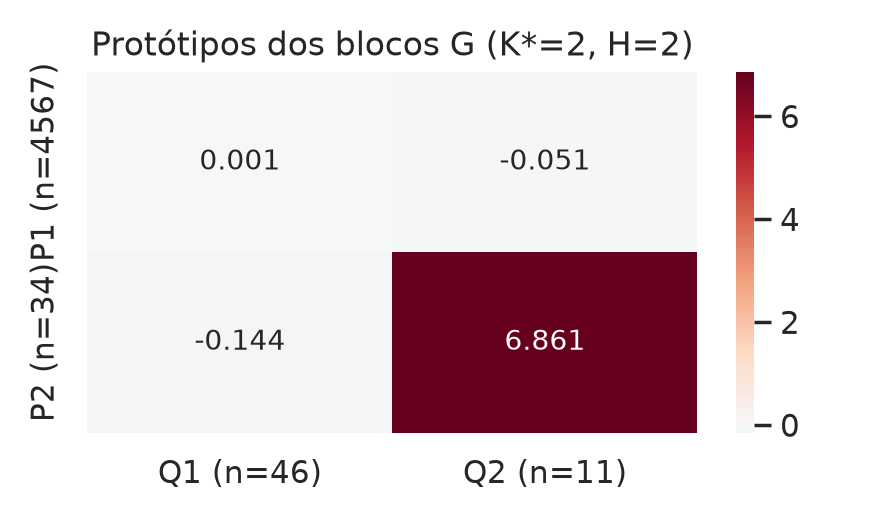
\includegraphics[width=0.45\textwidth]{resultados_versao_final/q1_matriz_G.png}
\caption{Protótipos dos blocos $G$.}
\label{fig:G}
\end{figure}

O bloco $(P_2,Q_2)$ tem protótipo de $6{,}86$ desvios-padrão, enquanto os outros ficam próximos
de zero. O grupo $P_2$ é formado por 34 e-mails que usam com frequência muito alta as palavras
de $Q_2$, típicas de mensagens internas do laboratório (HP Labs) onde a base foi coletada.

\subsubsection*{(ii) Matriz de confusão}

\begin{table}[H]
\centering
\caption{Partição do double k-means ($K^*=2$) $\times$ classe a priori.}
\label{tab:cm}
\begin{tabular}{lrrr}
\toprule
Cluster & Não-spam & Spam & Total \\
\midrule
$P_1$ & 2754 & 1813 & 4567 \\
$P_2$ & 34 & 0 & 34 \\
\midrule
Total & 2788 & 1813 & 4601 \\
\bottomrule
\end{tabular}
\end{table}

Os 34 e-mails de $P_2$ são todos legítimos, e $P_1$ reúne todos os 1813 spams junto com 2754
não-spams (Tabela~\ref{tab:cm} e Figura~\ref{fig:cm}).

\begin{figure}[H]
\centering
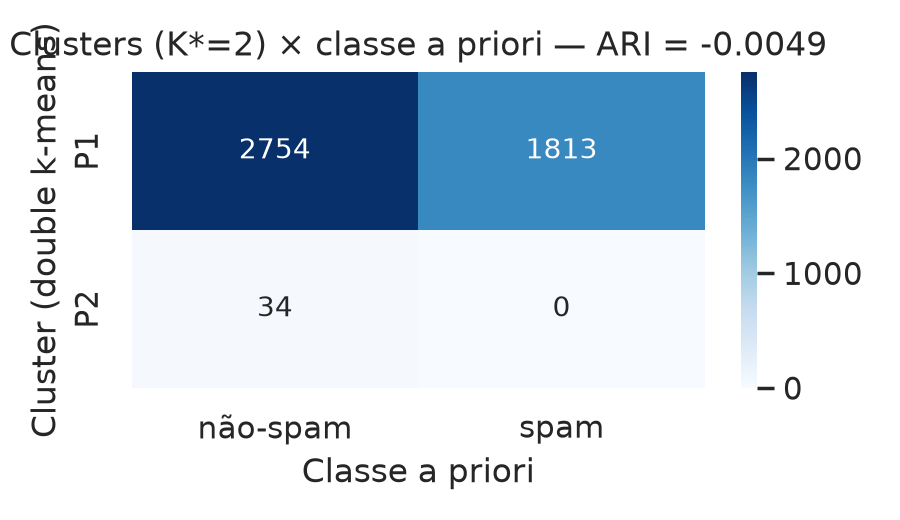
\includegraphics[width=0.5\textwidth]{resultados_versao_final/q1_matriz_confusao.png}
\caption{Matriz de confusão: clusters $\times$ classe a priori.}
\label{fig:cm}
\end{figure}

\subsubsection*{(iii) Função objetivo $\times$ iterações}
A Figura~\ref{fig:obj} mostra a função objetivo da melhor execução com $K^*=2$. Ela decresce
de forma monótona, de $262\,253{,}78$ na solução inicial para $244\,486{,}70$, e o algoritmo para
na iteração 40, quando não há mais transferências.

\begin{figure}[H]
\centering
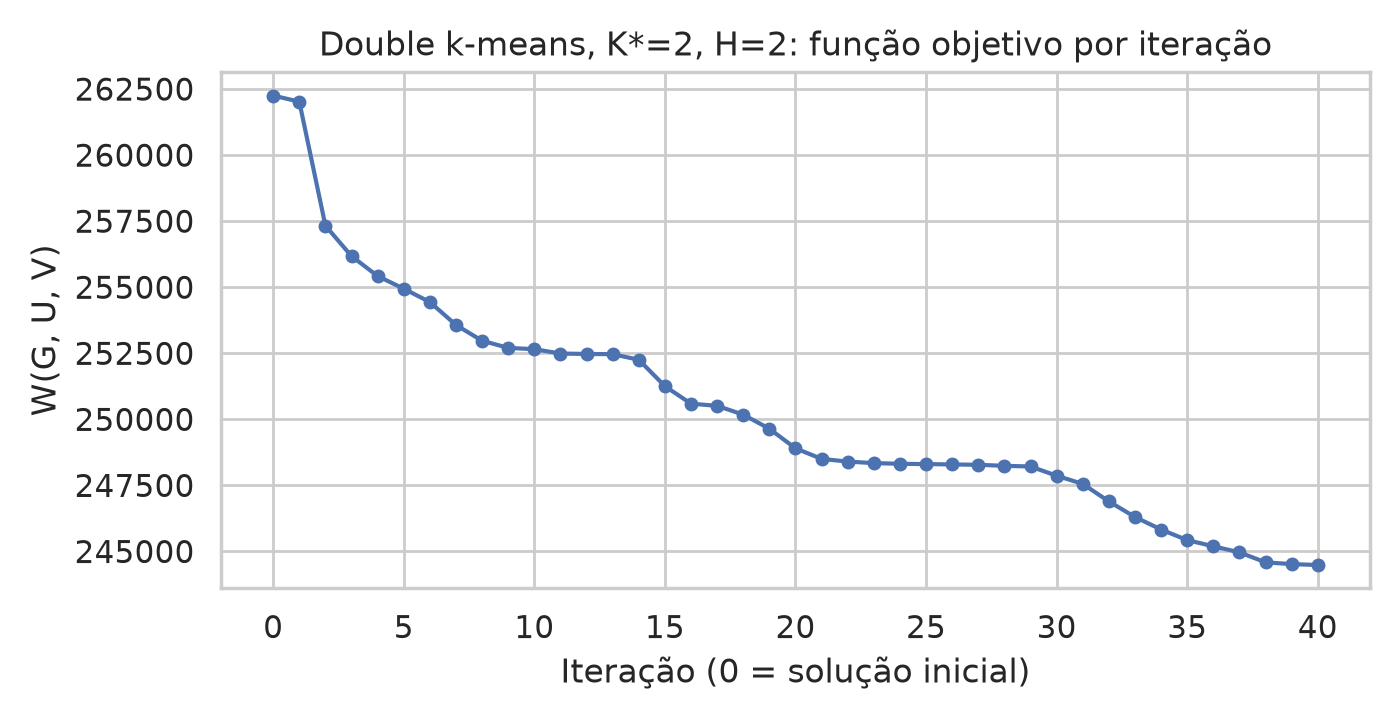
\includegraphics[width=0.8\textwidth]{resultados_versao_final/q1_objetivo_iteracoes.png}
\caption{Função objetivo $W$ por iteração (melhor execução, $K^*=2$, $H=2$).}
\label{fig:obj}
\end{figure}

\subsubsection*{Comentário}
A silhueta escolhe $K^*=2$ porque o par $(2,2)$ isola um grupo pequeno, extremo e bem separado
dos demais. Essa estrutura é real nos dados, mas não corresponde à divisão spam $\times$
não-spam, como mostram o ARI próximo de zero e a matriz de confusão. O resultado reflete
limitações do double k-means: sensibilidade a valores discrepantes e preferência por grupos
compactos e esféricos, numa base esparsa (a maioria dos atributos tem mais de 70\% de zeros) e
muito assimétrica. Também mostra que um índice interno alto (silhueta) não garante concordância
com as classes conhecidas (validação externa).

\subsection{Questão 2:}

\subsubsection*{Versões da base}
\begin{itemize}
\item \textbf{V1 (original):} classe \texttt{is\_spam}, 2 classes a priori (2788 não-spam e 1813 spam);
\item \textbf{V2 (clusters):} classe igual ao grupo do double k-means com $K^*=2$ (Questão~1),
  com 4567 e 34 exemplos.
\end{itemize}

\subsubsection*{Classificadores}
Em todos os classificadores bayesianos, $x_k$ é atribuído à classe de maior posteriori
$P(\omega_i\mid x_k)=p(x_k\mid\omega_i)P(\omega_i)/\sum_{r}p(x_k\mid\omega_r)P(\omega_r)$, com
$P(\omega_i)=n_i/n$ (máxima verossimilhança).
\begin{enumerate}
\item[(i)] \textbf{Bayesiano gaussiano:} $p(x_k\mid\omega_i)$ normal multivariada com
  $\hat\mu_i$ e $\hat\Sigma_i$ de máxima verossimilhança. Como alguns atributos são quase
  constantes dentro de uma classe, somou-se $10^{-3}I$ a $\hat\Sigma_i$ para que ela seja inversível.
\item[(ii)] \textbf{Bayesiano k-vizinhos:} $P(\omega_i\mid x)=k_i/k$, em que $k_i$ é o número de
  vizinhos da classe $\omega_i$ entre os $k$ mais próximos. Hiper-parâmetros: distância
  (Euclidiana, City-Block ou Chebyshev) e $k\in\{1,3,\dots,31\}$.
\item[(iii)] \textbf{Bayesiano janela de Parzen:} kernel multivariado produto de gaussianas
  univariadas,
  $p(x\mid\omega_i)=\frac{1}{n_i}\sum_{l\in\omega_i}\prod_{j=1}^{d}\frac{1}{h}\varphi\!\left(\frac{x_j-x_{lj}}{h}\right)$.
  Hiper-parâmetro: $h$, em 24 valores log-espaçados entre 0,1 e 20.
\item[(iv)] \textbf{Regressão logística:} multinomial com regularização L2. Hiper-parâmetro:
  $C\in\{10^{-3},10^{-2},\dots,10^{4}\}$.
\item[(v)] \textbf{Voto majoritário:} combina as predições de (i)--(iv). Em caso de empate,
  vence a classe de maior posteriori média.
\end{enumerate}

\subsubsection*{Organização dos experimentos}
\begin{itemize}
\item \textbf{Validação cruzada estratificada $30\times10$-folds:} em cada uma das 30
  repetições (sementes diferentes), a base é dividida em 10 folds estratificados. Cada fold é
  usado uma vez como teste, e os outros 9 formam o conjunto de aprendizagem. Isso dá 300
  avaliações por classificador e por versão. As partições são as mesmas para os 5
  classificadores, o que torna a comparação pareada.
\item \textbf{Ajuste de hiper-parâmetros:} dentro dos 9 folds de aprendizagem faz-se uma
  validação cruzada estratificada 5-folds. Escolhe-se a combinação de maior F-measure média nos
  5 folds internos, retreina-se o modelo nos 9 folds com esses valores e avalia-se no fold de
  teste, que nunca participa do ajuste.
\item \textbf{Padronização:} o \emph{z-score} é estimado só nos dados de treinamento de cada
  etapa, para que nenhuma informação do teste seja usada.
\item \textbf{Métricas:} taxa de erro, precisão, cobertura e F-measure. Na V1 a classe positiva
  é spam; na V2 usa-se a média \emph{macro} entre as classes.
\end{itemize}

\subsubsection*{Hiper-parâmetros selecionados}
A Tabela~\ref{tab:hp} mostra os valores mais escolhidos nos 300 folds externos. A
Figura~\ref{fig:hp} mostra a F-measure média da validação interna para cada valor.

\begin{table}[H]
\centering
\caption{Hiper-parâmetros mais selecionados (número de folds externos, em 300).}
\label{tab:hp}
\small
\begin{tabular}{lll}
\toprule
Classificador & V1 (original) & V2 (clusters) \\
\midrule
k-NN & City-Block, $k=1$ (99); & Euclidiana, $k=1$ (184); \\
     & City-Block, $k=5$ (94); & City-Block, $k=1$ (36) \\
     & Euclidiana, $k=1$ (54) & \\
Parzen & $h=0{,}50$ (245); $h=0{,}63$ (49) & $h=0{,}10$ (124); $h=1{,}00$ (49) \\
Reg. logística & $C=10$ (122); $C=100$ (95) & $C=0{,}1$ (176); $C=1$ (120) \\
\bottomrule
\end{tabular}
\end{table}

\begin{figure}[H]
\centering
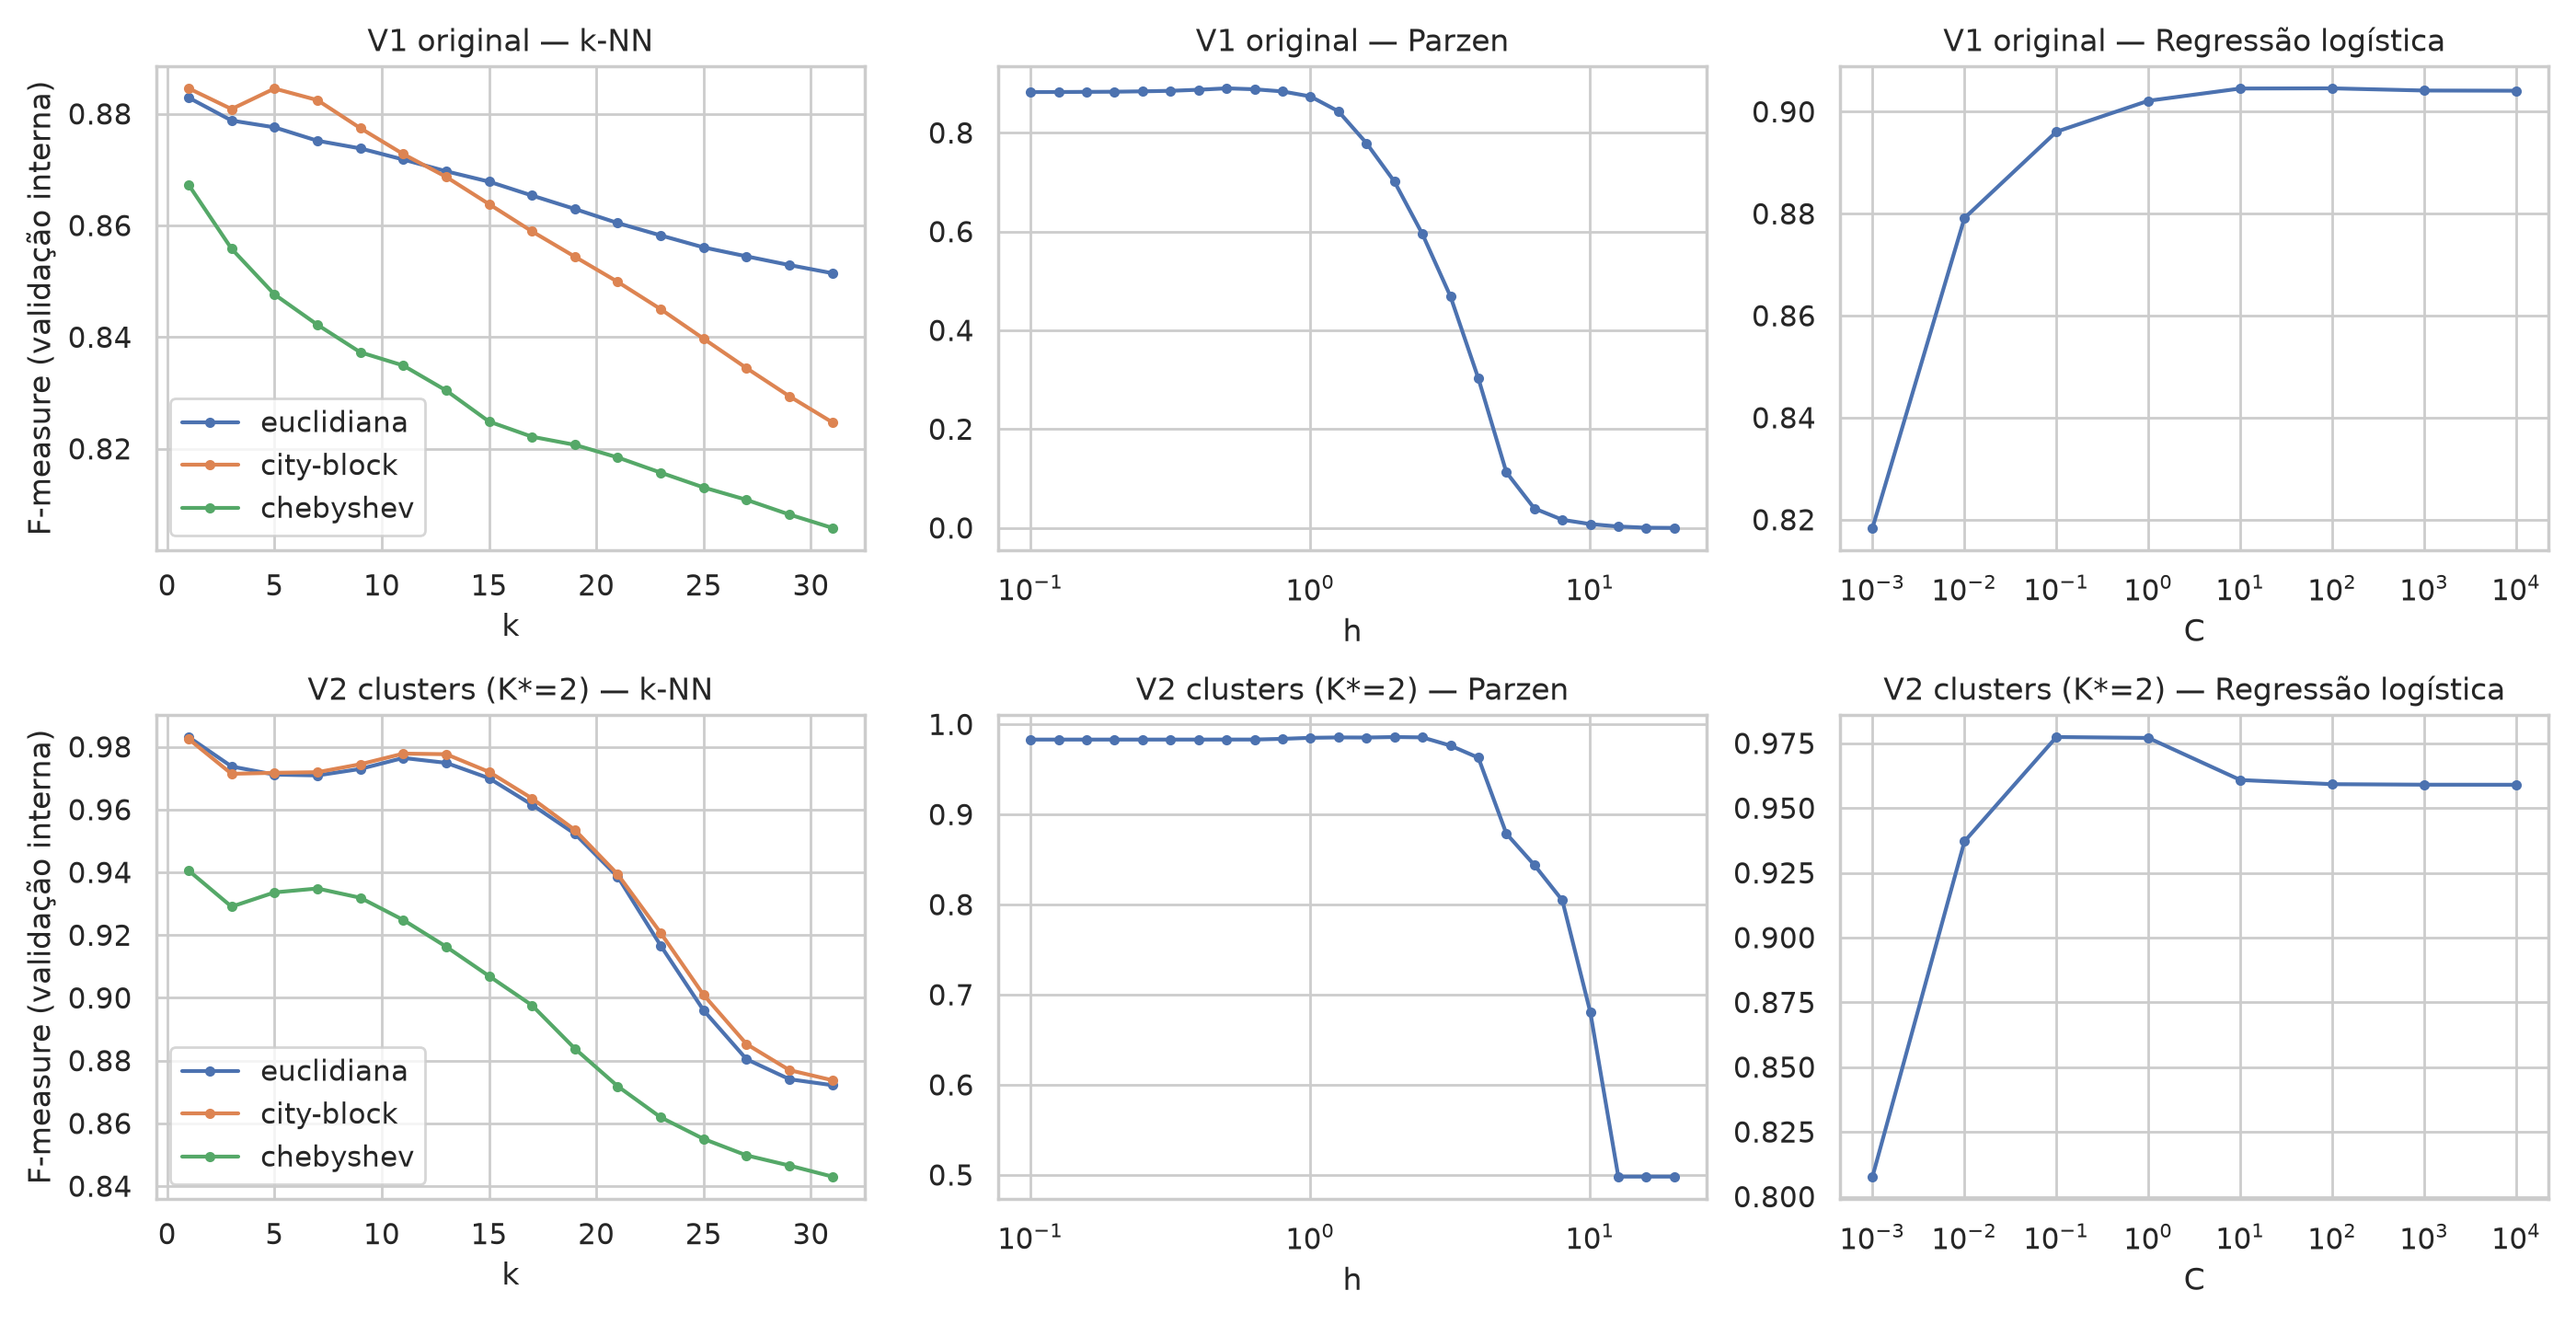
\includegraphics[width=\textwidth]{resultados_versao_final/q2_ajuste_hiperparametros.png}
\caption{F-measure média da validação interna (5-folds) em função de cada hiper-parâmetro.}
\label{fig:hp}
\end{figure}

\subsubsection*{(b) Estimativas pontuais e intervalos de confiança}
Para cada classificador e métrica, a média dos 10 folds de cada repetição dá 30 valores. A
estimativa pontual é a média desses 30 valores, e o intervalo de confiança de 95\% é
$\bar m \pm t_{0{,}975;29}\, s/\sqrt{30}$. Usam-se as médias por repetição porque os folds de uma
mesma repetição compartilham dados de treino e não são independentes. Os resultados estão nas
Tabelas~\ref{tab:icv1} e~\ref{tab:icv2} e na Figura~\ref{fig:ic}.

\begin{table}[H]
\centering
\caption{V1 (original): média e IC 95\%.}
\label{tab:icv1}
\resizebox{\textwidth}{!}{%
\begin{tabular}{lcccc}
\toprule
Classificador & Taxa de erro & Precisão & Cobertura & F-measure \\
\midrule
Gaussiano & 0,1767 [0,1763; 0,1770] & 0,7052 [0,7048; 0,7057] & \textbf{0,9499} [0,9494; 0,9504] & 0,8092 [0,8089; 0,8096] \\
k-NN & 0,0861 [0,0851; 0,0871] & 0,9121 [0,9101; 0,9141] & 0,8658 [0,8632; 0,8684] & 0,8878 [0,8864; 0,8892] \\
Parzen & 0,0792 [0,0786; 0,0798] & 0,9138 [0,9129; 0,9147] & 0,8826 [0,8812; 0,8840] & 0,8977 [0,8969; 0,8985] \\
Reg. logística & 0,0732 [0,0728; 0,0735] & \textbf{0,9229} [0,9221; 0,9237] & 0,8891 [0,8883; 0,8899] & 0,9054 [0,9049; 0,9059] \\
Voto majoritário & \textbf{0,0655} [0,0648; 0,0661] & 0,9184 [0,9172; 0,9195] & 0,9157 [0,9145; 0,9169] & \textbf{0,9168} [0,9160; 0,9176] \\
\bottomrule
\end{tabular}}
\end{table}

\begin{table}[H]
\centering
\caption{V2 (clusters, $K^*=2$): média e IC 95\%.}
\label{tab:icv2}
\resizebox{\textwidth}{!}{%
\begin{tabular}{lcccc}
\toprule
Classificador & Taxa de erro & Precisão & Cobertura & F-measure \\
\midrule
Gaussiano & 0,0459 [0,0457; 0,0462] & 0,5561 [0,5550; 0,5571] & 0,8524 [0,8471; 0,8577] & 0,5866 [0,5850; 0,5882] \\
k-NN & 0,0008 [0,0007; 0,0008] & \textbf{0,9812} [0,9785; 0,9838] & 0,9720 [0,9695; 0,9746] & 0,9726 [0,9709; 0,9743] \\
Parzen & 0,0005 [0,0004; 0,0005] & 0,9796 [0,9774; 0,9818] & 0,9956 [0,9924; 0,9989] & 0,9856 [0,9828; 0,9883] \\
Reg. logística & 0,0007 [0,0006; 0,0008] & 0,9680 [0,9646; 0,9714] & 0,9955 [0,9922; 0,9988] & 0,9789 [0,9759; 0,9818] \\
Voto majoritário & \textbf{0,0004} [0,0003; 0,0005] & 0,9807 [0,9782; 0,9832] & \textbf{0,9973} [0,9945; 1,0000] & \textbf{0,9872} [0,9846; 0,9898] \\
\bottomrule
\end{tabular}}
\end{table}

\begin{figure}[H]
\centering
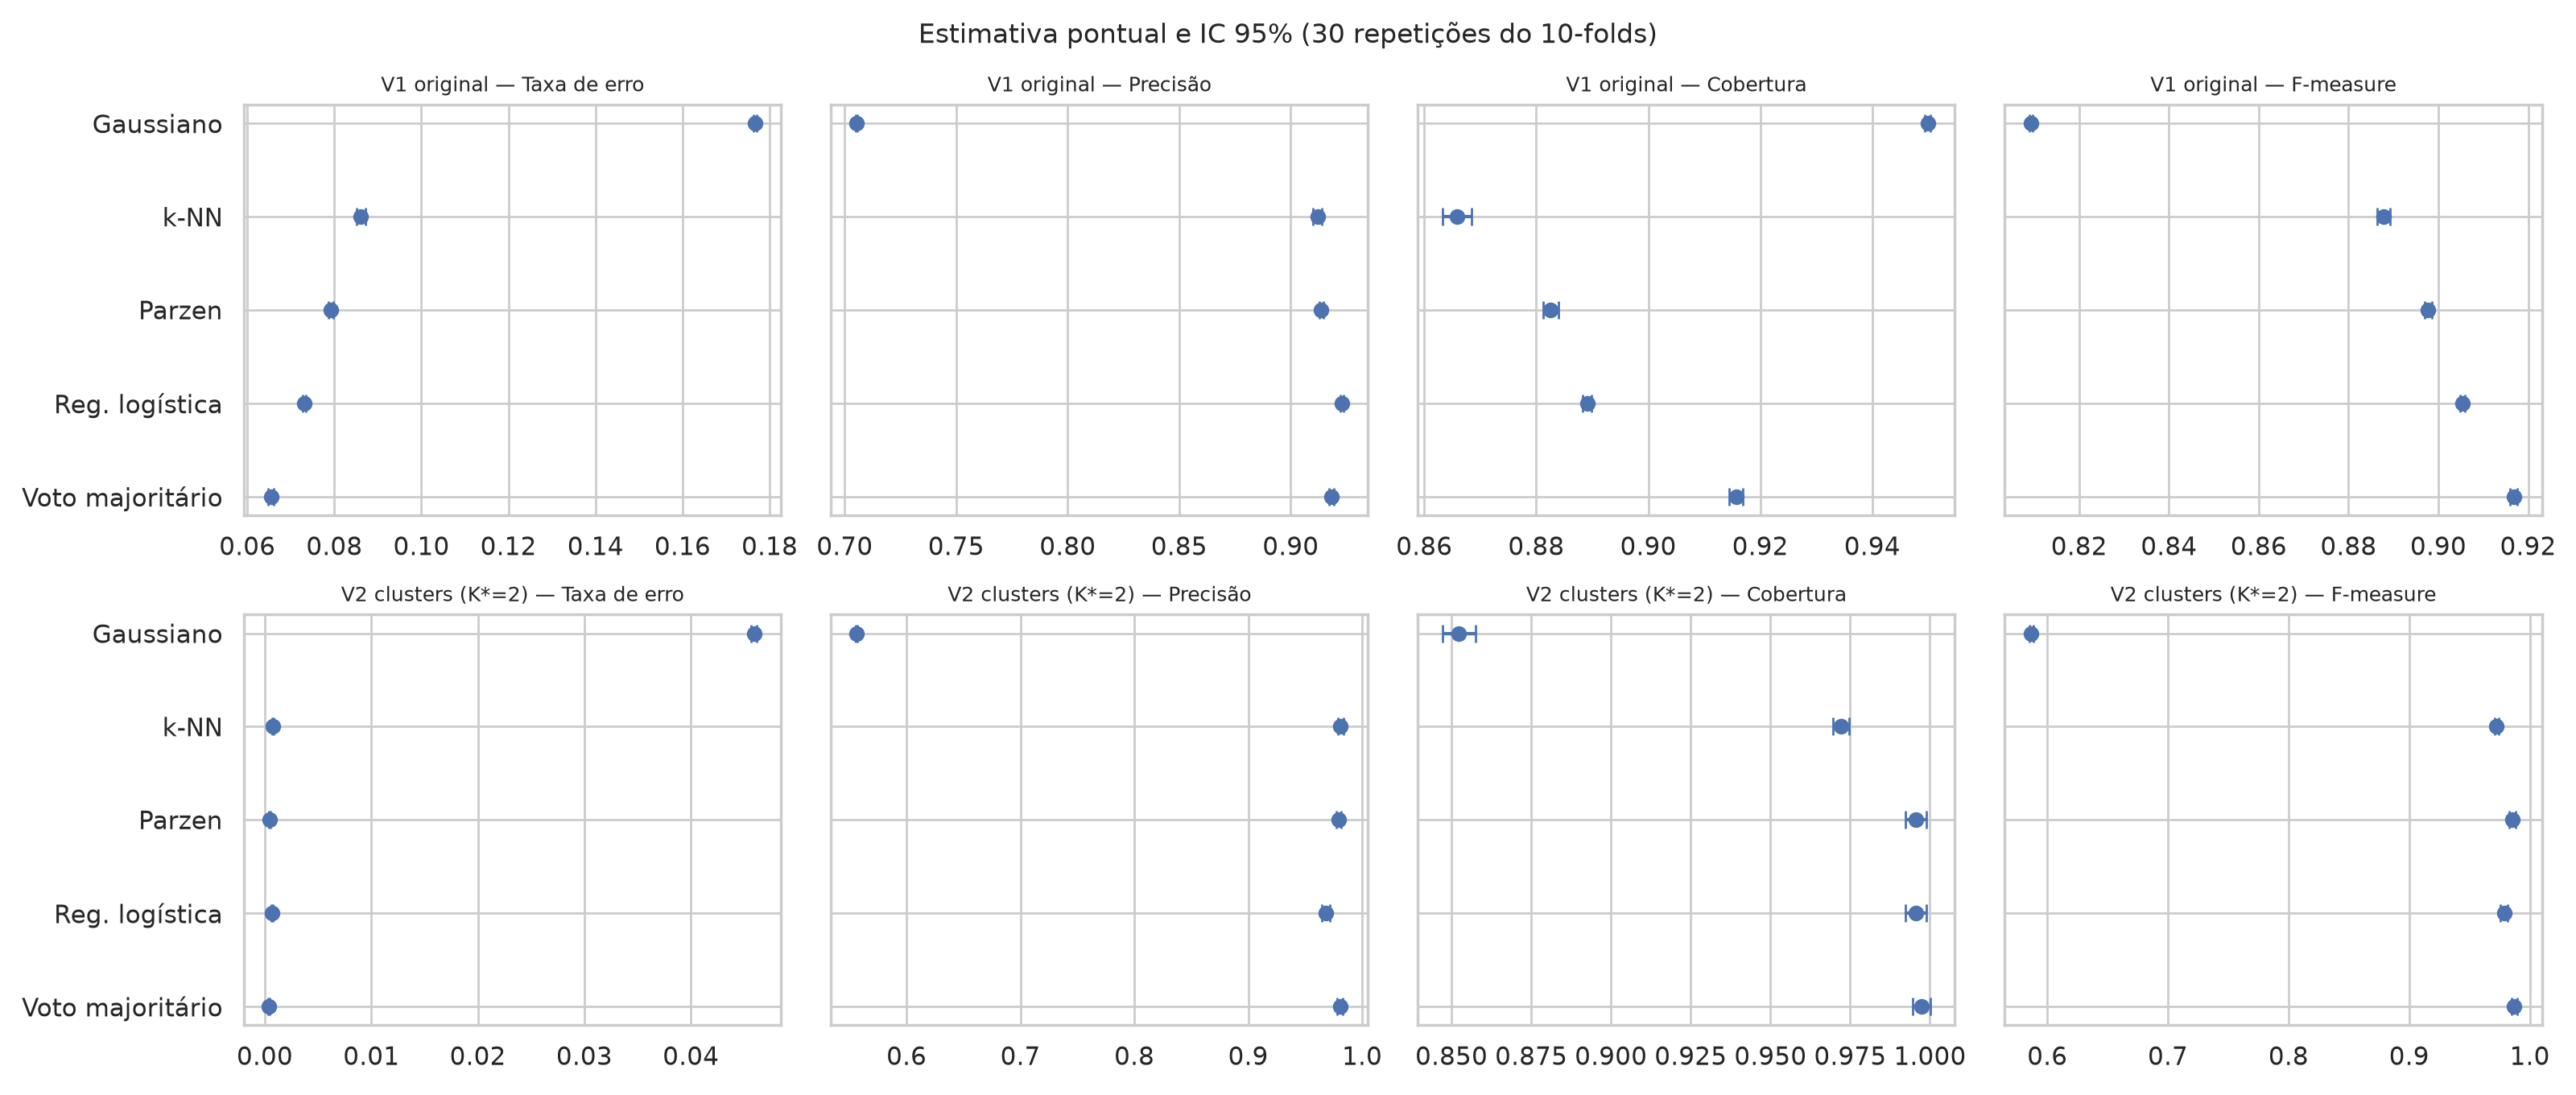
\includegraphics[width=\textwidth]{resultados_versao_final/q2_ic95.png}
\caption{Estimativas pontuais e IC 95\% (linha superior: V1; inferior: V2).}
\label{fig:ic}
\end{figure}

Na V1, o voto majoritário tem a menor taxa de erro (6,55\%) e a maior F-measure (0,917), seguido
pela regressão logística, Parzen e k-NN. O bayesiano gaussiano é o pior em erro (17,7\%), mas tem
a maior cobertura (0,950) com precisão baixa (0,705): ele classifica muitos e-mails legítimos
como spam, porque a hipótese de normalidade é ruim para atributos esparsos e de cauda pesada. Na
V2 a tarefa é muito mais fácil, porque as classes foram definidas pelo próprio agrupamento a
partir de um grupo extremo em poucas variáveis. O erro fica abaixo de 0,1\% para todos os
classificadores, exceto o gaussiano (4,6\%; F-measure 0,587): estimar uma matriz de covariância
$57\times57$ com cerca de 31 exemplos de treino da classe minoritária é mal condicionado.

\subsubsection*{(c) Teste de Friedman e pós-teste de Nemenyi}
Para cada versão e métrica, os blocos são as 30 repetições e os tratamentos são os 5
classificadores. O posto 1 indica o melhor classificador. A diferença crítica de Nemenyi
($\alpha=0{,}05$, $k=5$, $N=30$) é $CD=q_\alpha\sqrt{k(k+1)/(6N)}=1{,}114$.

\begin{table}[H]
\centering
\caption{Teste de Friedman e postos médios (1 = melhor).}
\label{tab:friedman}
\resizebox{\textwidth}{!}{%
\begin{tabular}{llrcccccc}
\toprule
Base & Métrica & $\chi^2_F$ & $p$-valor & Gaussiano & k-NN & Parzen & Reg. log. & Voto \\
\midrule
\multirow{4}{*}{V1} & Taxa de erro & 120,00 & $5{,}3\times10^{-25}$ & 5,00 & 4,00 & 3,00 & 2,00 & 1,00 \\
 & Precisão  & 108,51 & $1{,}5\times10^{-22}$ & 5,00 & 3,57 & 3,33 & 1,10 & 2,00 \\
 & Cobertura & 118,51 & $1{,}1\times10^{-24}$ & 1,00 & 5,00 & 3,93 & 3,07 & 2,00 \\
 & F-measure & 120,00 & $5{,}3\times10^{-25}$ & 5,00 & 4,00 & 3,00 & 2,00 & 1,00 \\
\midrule
\multirow{4}{*}{V2} & Taxa de erro & 97,10 & $4{,}1\times10^{-20}$ & 5,00 & 3,40 & 1,90 & 3,12 & 1,58 \\
 & Precisão  & 94,04 & $1{,}8\times10^{-19}$ & 5,00 & 2,75 & 1,92 & 3,65 & 1,68 \\
 & Cobertura & 98,18 & $2{,}4\times10^{-20}$ & 5,00 & 3,75 & 1,97 & 2,68 & 1,60 \\
 & F-measure & 98,26 & $2{,}3\times10^{-20}$ & 5,00 & 3,60 & 1,88 & 2,97 & 1,55 \\
\bottomrule
\end{tabular}}
\end{table}

O teste de Friedman rejeita a hipótese de desempenhos equivalentes em todas as métricas e nas
duas versões ($p<10^{-18}$). Resultados do pós-teste de Nemenyi (Figuras~\ref{fig:nemenyi}
e~\ref{fig:postos}):
\begin{itemize}
\item \textbf{V1, taxa de erro e F-measure:} a ordem voto $<$ reg. logística $<$ Parzen $<$
  k-NN $<$ gaussiano é a mesma nas 30 repetições. Classificadores vizinhos nessa ordem não
  diferem significativamente (diferença de posto 1,0 $<$ CD; $p=0{,}10$). Pares a duas ou mais
  posições de distância diferem ($p<0{,}001$): por exemplo, o voto supera Parzen, k-NN e
  gaussiano, e a regressão logística supera k-NN e gaussiano.
\item \textbf{V1, precisão:} regressão logística e voto formam o melhor grupo (sem diferença
  entre si, $p=0{,}18$) e superam os demais. \textbf{Cobertura:} o gaussiano é o melhor, sem
  diferença significativa para o voto ($p=0{,}10$).
\item \textbf{V2:} voto e Parzen não diferem entre si em nenhuma métrica ($p\ge0{,}90$) e superam
  k-NN e gaussiano. Na F-measure, o voto também supera a regressão logística ($p=0{,}005$). O
  gaussiano é significativamente o pior em todas as métricas.
\end{itemize}

\begin{figure}[H]
\centering
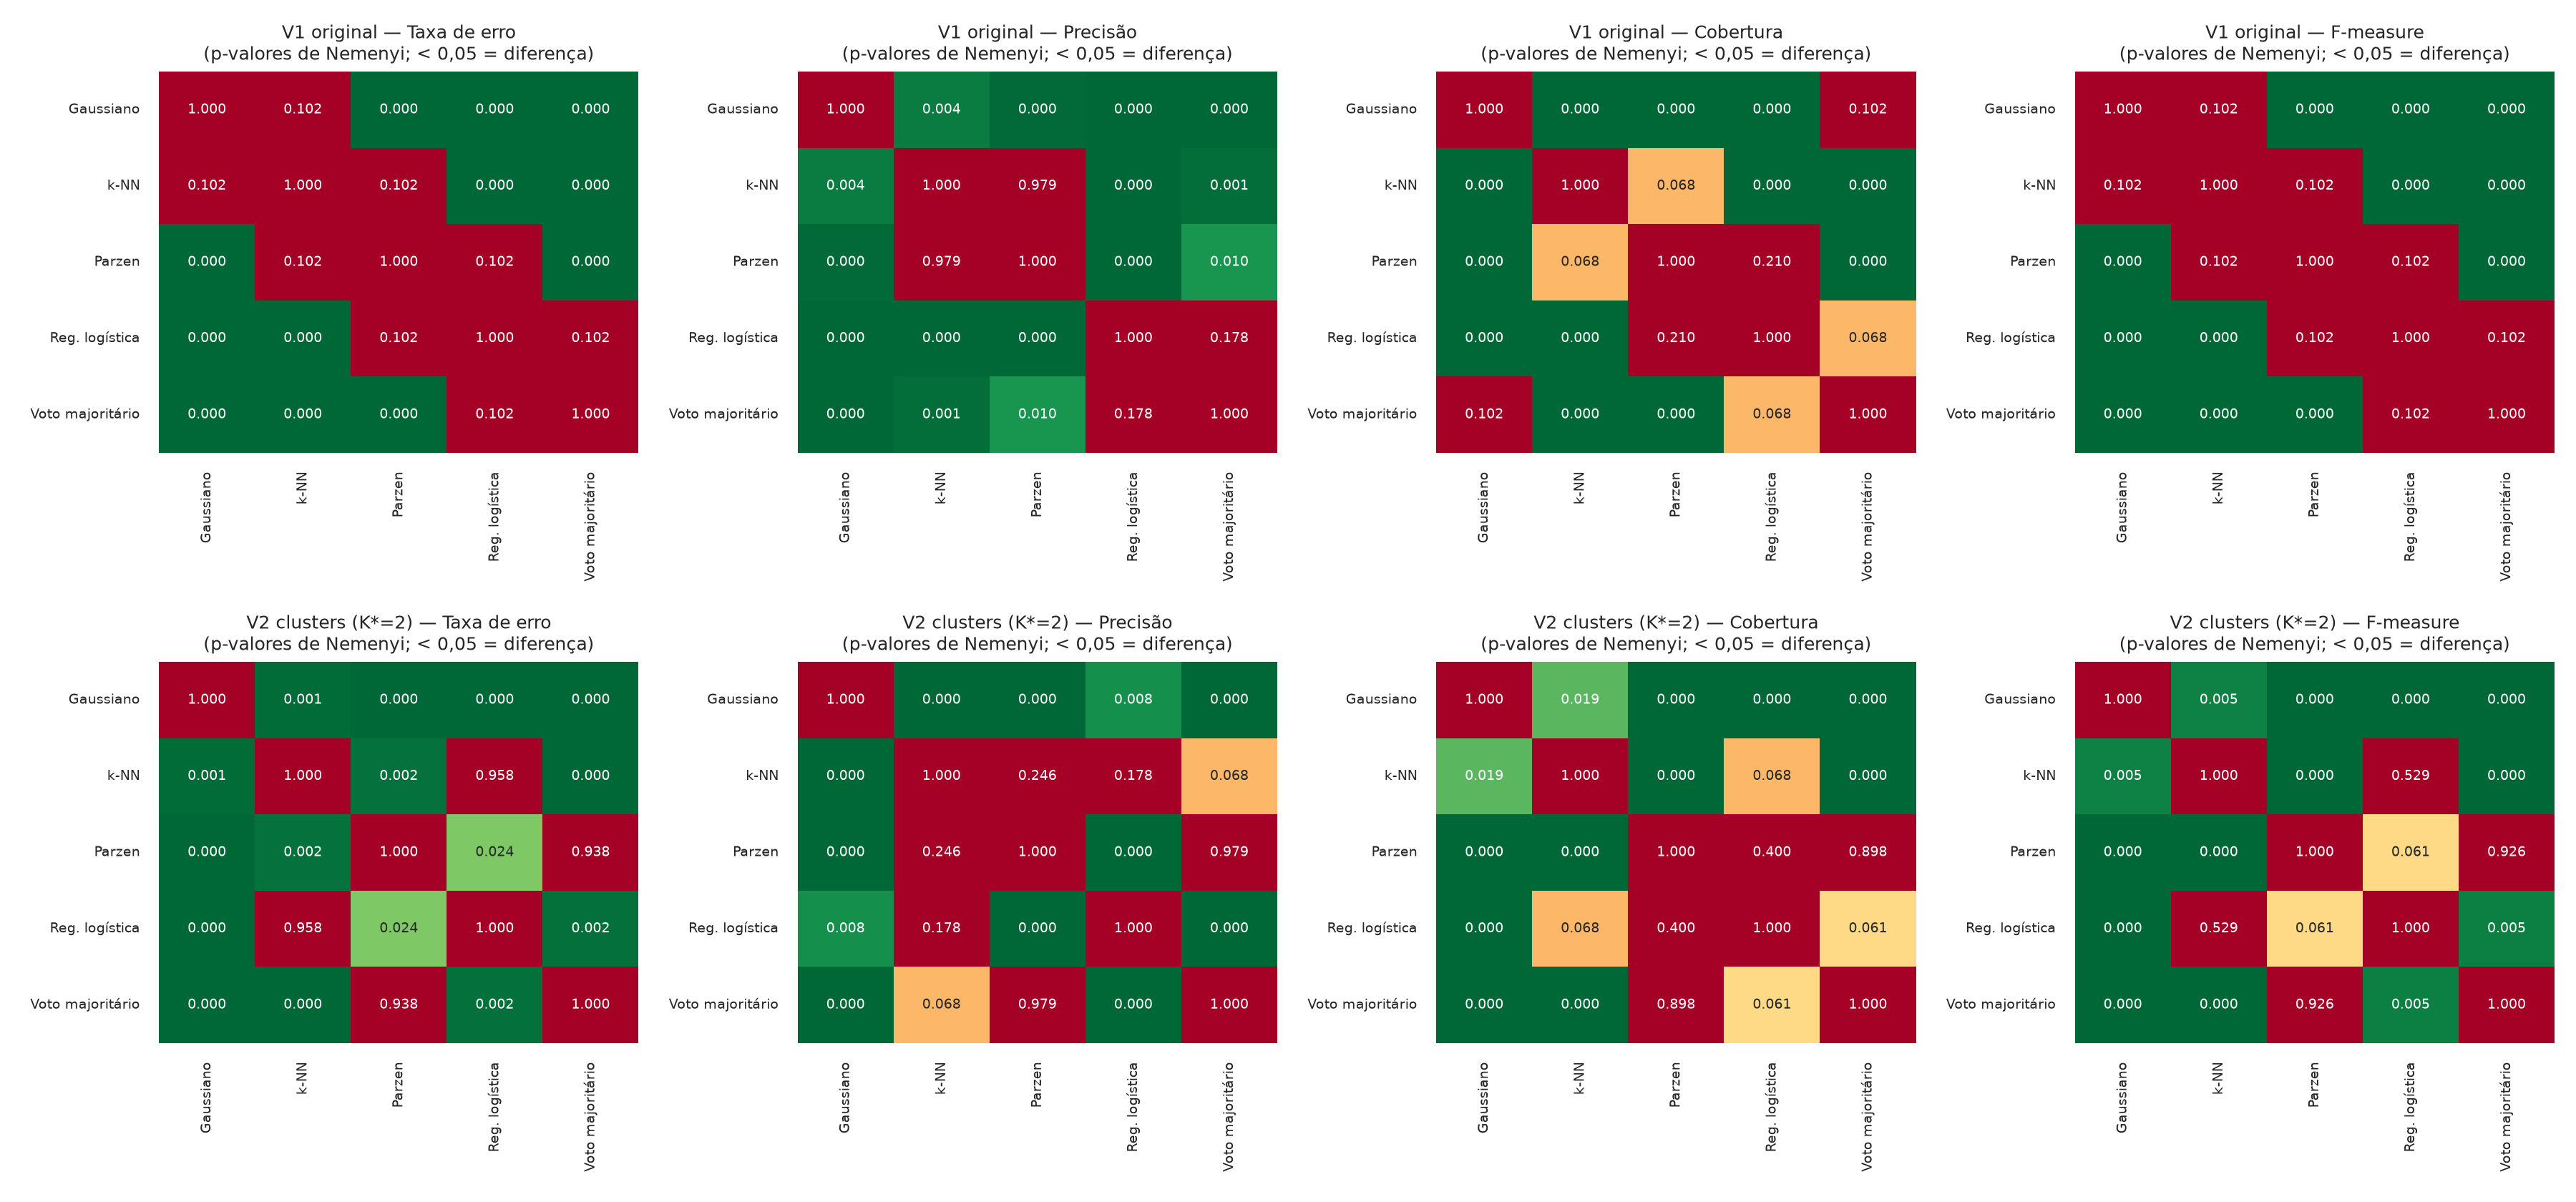
\includegraphics[width=\textwidth]{resultados_versao_final/q2_nemenyi.png}
\caption{$p$-valores do pós-teste de Nemenyi (valores $<0{,}05$ indicam diferença significativa).}
\label{fig:nemenyi}
\end{figure}

\begin{figure}[H]
\centering
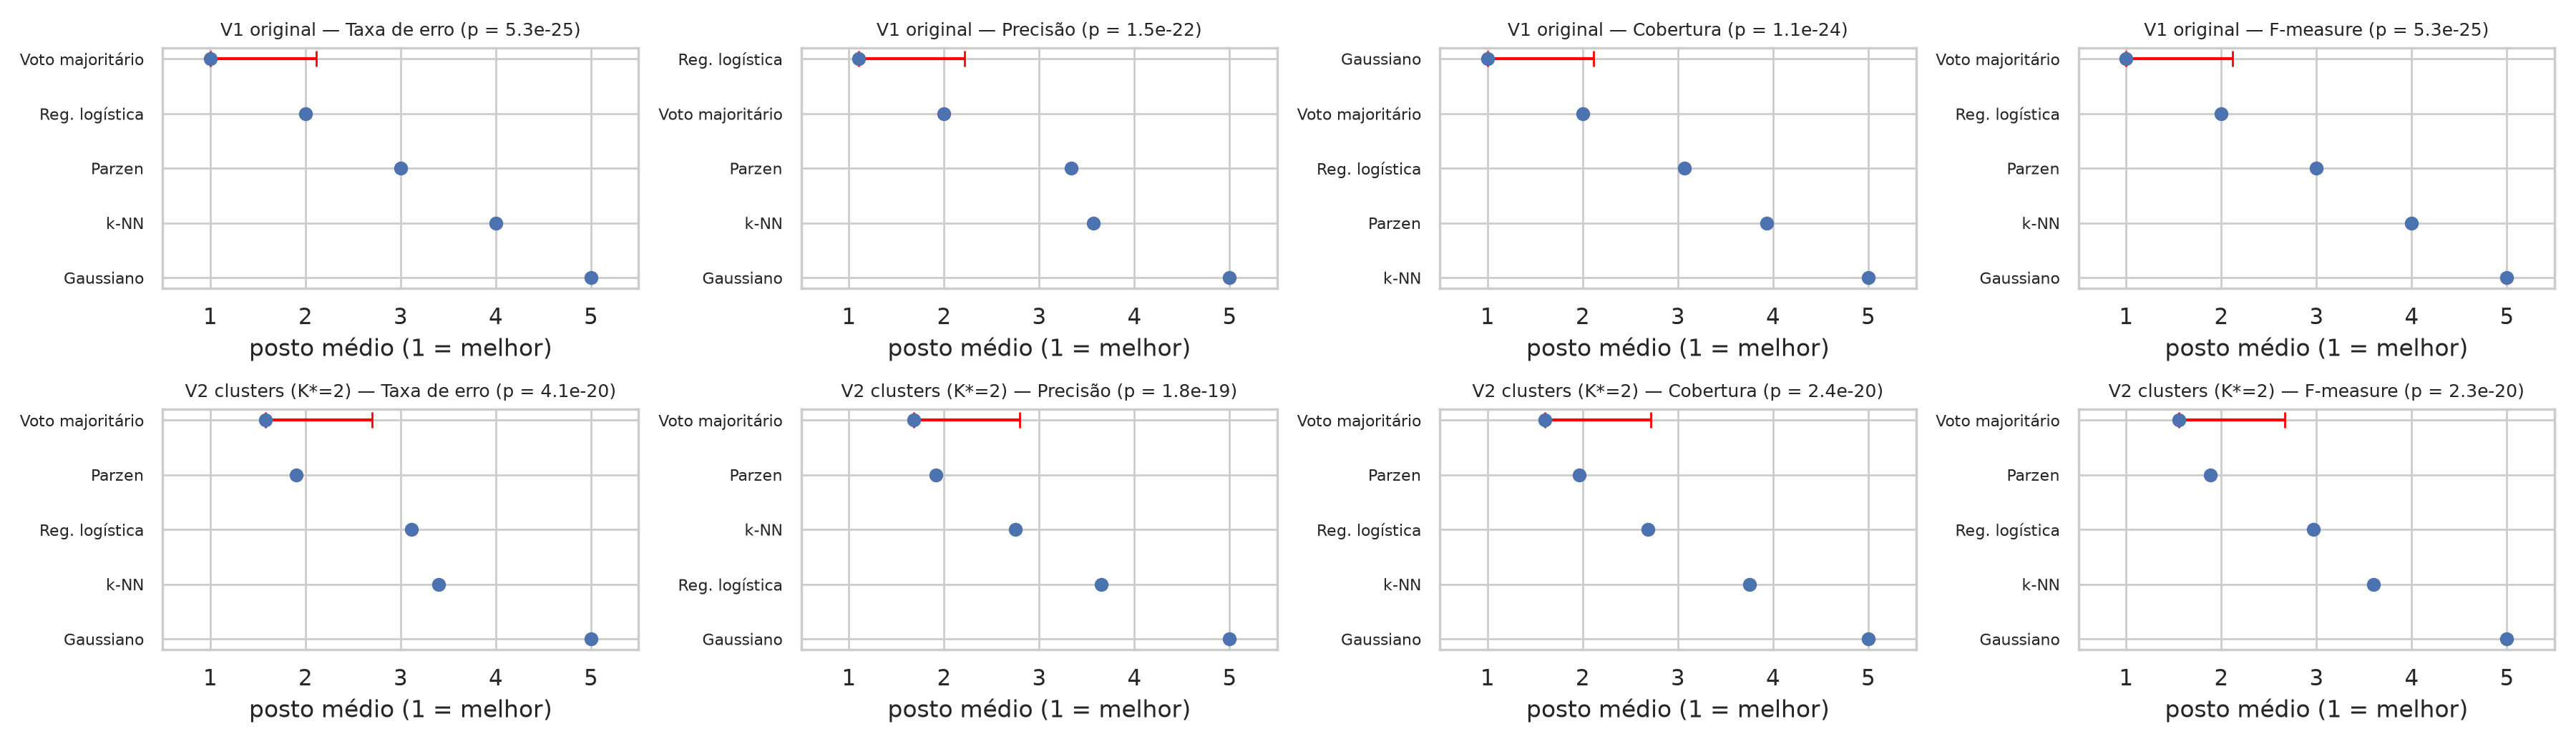
\includegraphics[width=\textwidth]{resultados_versao_final/q2_postos_medios.png}
\caption{Postos médios dos classificadores; a barra vermelha indica a diferença crítica (CD).}
\label{fig:postos}
\end{figure}

\subsubsection*{(d) Curvas de aprendizagem}
Para proporções de treinamento de 5\% a 95\% (passo de 5\%), a base foi dividida em treino e
teste por amostragem estratificada. Os classificadores usaram os hiper-parâmetros mais
selecionados no item (a): na V1, City-Block com $k=1$, $h=0{,}50$ e $C=10$; na V2, Euclidiana
com $k=1$, $h=0{,}10$ e $C=0{,}1$. Cada proporção foi repetida 5 vezes, e a Figura~\ref{fig:lc}
mostra a F-measure média no treino e no teste.

\begin{figure}[H]
\centering
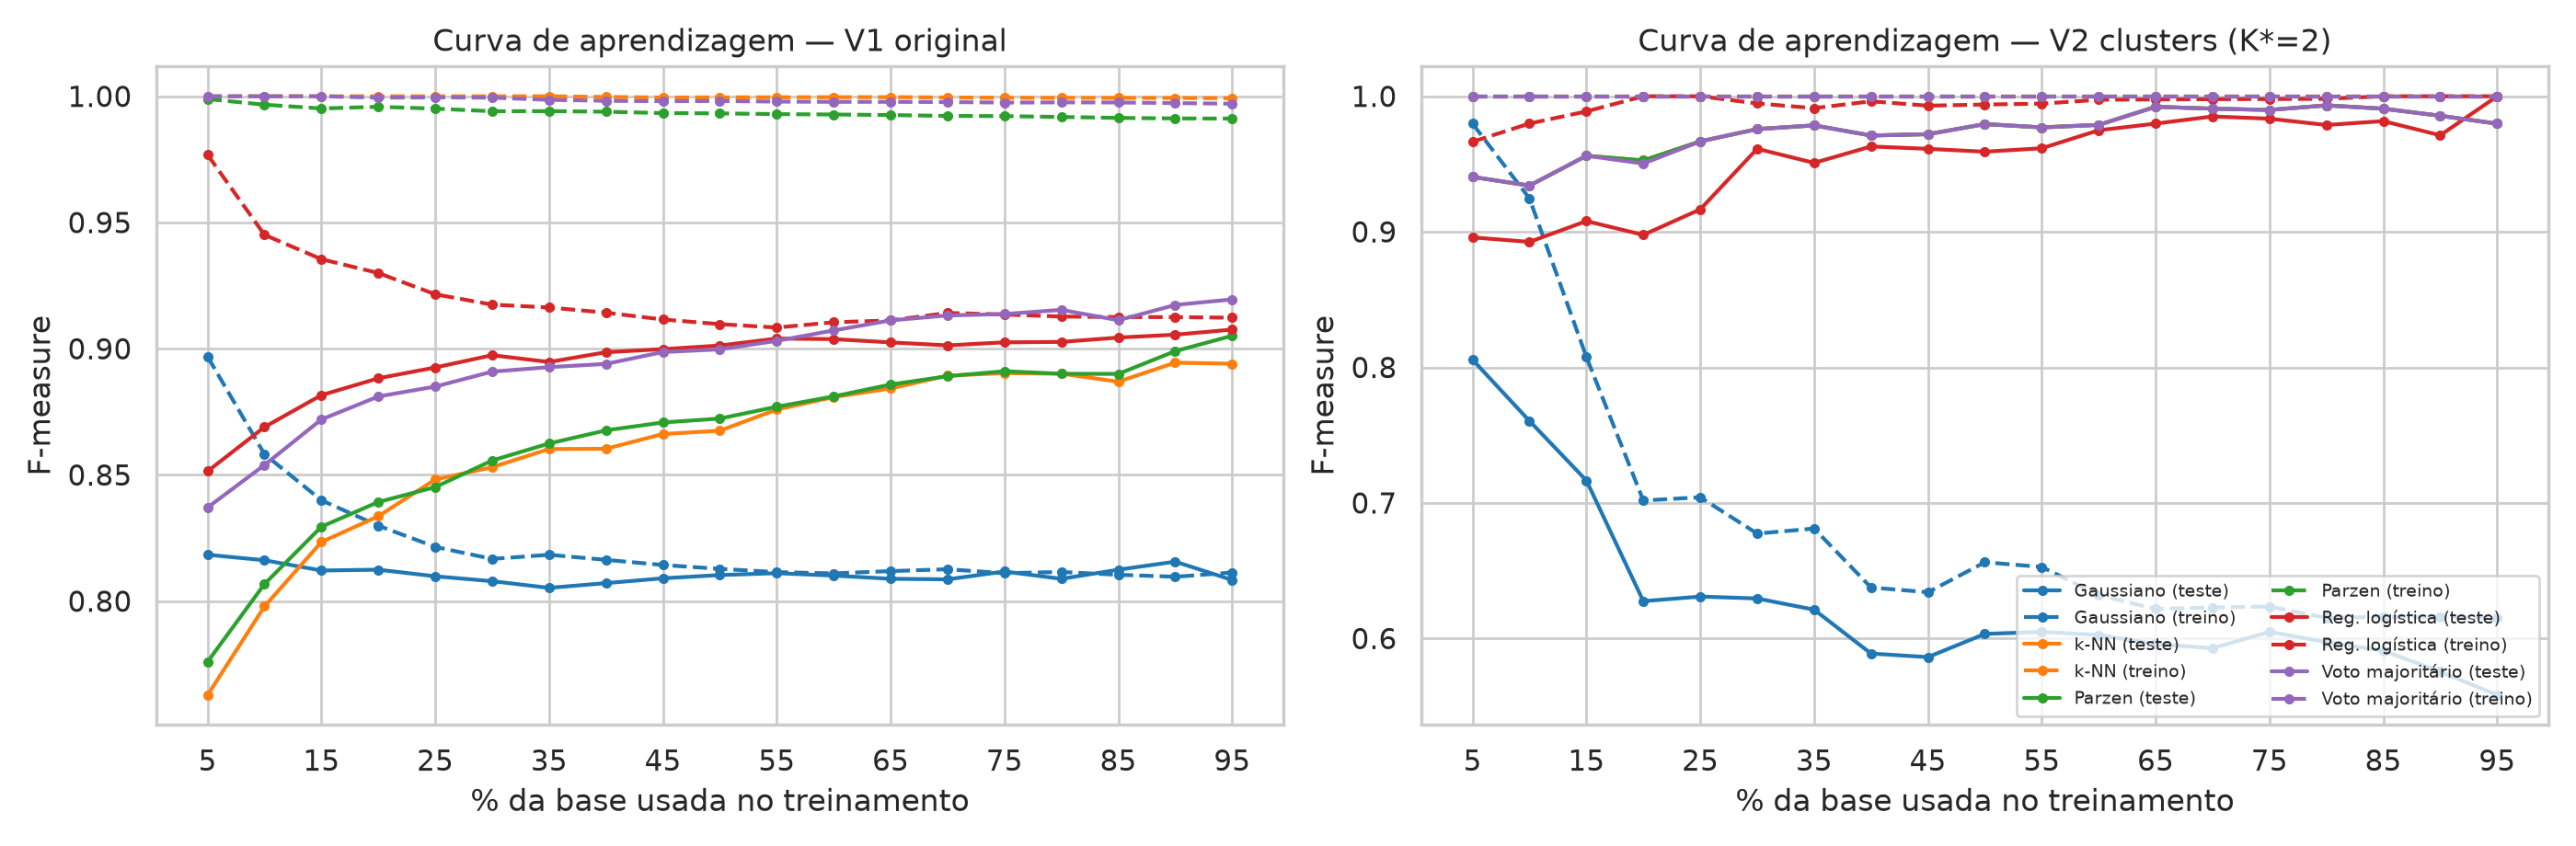
\includegraphics[width=\textwidth]{resultados_versao_final/q2_curva_aprendizagem_f1.png}
\caption{Curvas de aprendizagem da F-measure (linha cheia: teste; tracejada: treino).}
\label{fig:lc}
\end{figure}

\begin{itemize}
\item \textbf{V1:} k-NN e Parzen têm F-measure de treino próxima de 1, porque com $k=1$ e $h$
  pequeno eles memorizam o treino. A F-measure de teste cresce com o tamanho do treino (de 0,76
  para 0,89 no k-NN e de 0,78 para 0,91 no Parzen): são modelos de \textbf{alta variância}, que
  melhoram com mais dados. A regressão logística tem treino e teste próximos ($\approx0{,}91$ a
  partir de 25\%), ou seja, baixa variância. O gaussiano fica estável em $\approx0{,}81$ no treino
  e no teste: \textbf{alto viés}, e mais dados não o melhoram. Com treino grande, o voto
  majoritário é o melhor no teste (0,920 com 95\%).
\item \textbf{V2:} k-NN, Parzen e voto têm curvas praticamente iguais (de 0,94 para 0,98). A
  regressão logística chega a 1,0 com 95\% de treino. O gaussiano piora à medida que o treino
  cresce (de 0,81 para 0,56), coerente com a dificuldade de modelar a classe minoritária, muito
  pequena e dispersa, por uma normal multivariada.
\end{itemize}

\subsubsection*{Observações}
Os intervalos de confiança são estreitos porque cada um vem da média de 30 repetições do
10-folds sobre a mesma base. Eles medem a variabilidade da divisão em folds, não a de amostrar
novos conjuntos de dados. Na V2, o $h$ de Parzen mais escolhido foi o menor valor da grade
(0,1). Como o erro já é próximo de zero, isso não deve alterar as conclusões.

\section{Resultados e Discussão}

Esta seção reúne os principais resultados das duas questões, discute como eles se relacionam e
aponta as limitações do estudo. Os números detalhados estão na Seção~4.

\subsection*{Síntese dos resultados}

\begin{table}[H]
\centering
\caption{Resumo dos principais resultados.}
\label{tab:sintese}
\small
\begin{tabular}{p{0.27\textwidth}p{0.62\textwidth}}
\toprule
Item & Resultado \\
\midrule
Escolha de $K^*$ (Q1) & $(K,H)=(2,2)$, silhueta $0{,}660$; $K^*=2$ \\
Partição de $K^*$ (Q1) & Grupos de 4567 e 34 e-mails; ARI $=-0{,}005$ \\
Melhor classificador, V1 & Voto majoritário: erro $6{,}55\%$, F-measure $0{,}917$ \\
Pior classificador, V1 & Gaussiano: erro $17{,}67\%$, precisão $0{,}705$ \\
Melhor classificador, V2 & Voto majoritário: erro $0{,}04\%$, F-measure macro $0{,}987$ \\
Testes estatísticos & Friedman rejeita $H_0$ em todos os casos ($p<10^{-18}$); $CD=1{,}114$ \\
Tempo de execução & 42,6 min no total (GPU A100 + 16 CPUs) \\
\bottomrule
\end{tabular}
\end{table}

\subsection*{Agrupamento e classes conhecidas}
O resultado central da Questão~1 é que a melhor partição segundo a silhueta não tem relação
com a classe spam/não-spam (ARI $\approx 0$). O double k-means encontrou uma estrutura real: um
grupo de 34 e-mails internos da HP Labs que usam com frequência muito alta um conjunto de 11
palavras (\texttt{hp}, \texttt{lab}, \texttt{telnet}, \texttt{650}, \dots). Por ser pequeno, extremo
e bem separado do resto, esse grupo produz uma silhueta alta. Três fatores explicam o resultado:
\begin{itemize}
\item \textbf{Sensibilidade a \emph{outliers}:} a função objetivo é uma soma de erros
  quadráticos, então poucos e-mails com valores muito altos pesam bastante na partição;
\item \textbf{Esparsidade e assimetria:} com 77\% de zeros e caudas longas, a padronização
  z-score não deixa as variáveis com distribuições parecidas e amplia os valores extremos;
\item \textbf{Critério de escolha:} a silhueta mede compacidade e separação, não concordância
  com classes externas. Uma partição com um grupo minúsculo e isolado pode ter silhueta alta.
\end{itemize}
Os outros pares $(K,H)$ também tendem a isolar grupos pequenos (de 22 a 34 e-mails) ao lado de
grupos grandes (Tabela~\ref{tab:q1}). Isso mostra que a estrutura dominante da base, para esse
algoritmo, não é a divisão spam $\times$ não-spam. O exercício ilustra uma lição importante:
índices internos de validação não substituem a validação externa quando há classes conhecidas.

\subsection*{Desempenho dos classificadores}
Na base original (V1), a ordem dos classificadores foi a mesma em todas as 30 repetições: voto
majoritário, regressão logística, Parzen, k-NN e gaussiano. Os resultados mais relevantes:
\begin{itemize}
\item \textbf{O voto majoritário foi o melhor.} Combinar classificadores com vieses diferentes
  (um paramétrico linear, dois não paramétricos e um gaussiano) reduz os erros individuais. A
  diferença para a regressão logística (0,77 ponto percentual de erro) não foi significativa no
  Nemenyi, mas a vantagem sobre Parzen, k-NN e gaussiano foi.
\item \textbf{A regressão logística foi o melhor classificador individual.} Ela é simples, tem
  baixa variância e alcançou a maior precisão (0,923), o que é desejável em filtros de spam, onde
  marcar um e-mail legítimo como spam custa caro.
\item \textbf{Os métodos não paramétricos (k-NN e Parzen)} ficaram em posição intermediária. As
  curvas de aprendizagem indicam alta variância: eles melhoram à medida que o treino cresce e
  provavelmente se beneficiariam de mais dados ou de redução de dimensionalidade.
\item \textbf{O bayesiano gaussiano foi o pior.} A hipótese de normalidade multivariada é
  inadequada para atributos esparsos, limitados em zero e de cauda longa. Ele classifica spam
  em excesso (cobertura de 0,950 com precisão de 0,705) e tem alto viés: o desempenho não melhora
  com mais dados.
\end{itemize}

Na versão com as classes vindas do agrupamento (V2), todos os classificadores, exceto o
gaussiano, erram menos de 0,1\%. A tarefa é fácil porque as classes foram definidas pelo
próprio double k-means a partir de um grupo extremo em poucas variáveis. Assim, os resultados da
V2 mostram principalmente que a partição da Questão~1 é bem separada no espaço dos atributos.
Eles não indicam que esses classificadores sejam bons para detectar spam. O mau desempenho do
gaussiano na V2 vem do desbalanceamento extremo (4567 $\times$ 34): estimar uma covariância
$57\times57$ com cerca de 31 exemplos é mal condicionado, mesmo com regularização.

\subsection*{Validade dos experimentos}
O protocolo foi desenhado para que a avaliação e a comparação sejam justas:
\begin{itemize}
\item os hiper-parâmetros foram escolhidos só com os dados de aprendizagem (5-fold interno), e o
  fold de teste nunca participou do ajuste nem da padronização;
\item os 5 classificadores usaram exatamente as mesmas partições, o que permite testes
  pareados (Friedman e Nemenyi);
\item a amostragem estratificada preservou a proporção das classes em todas as divisões.
\end{itemize}

\subsection*{Limitações}
\begin{itemize}
\item \textbf{Independência:} as 30 repetições usam a mesma base, então os intervalos de
  confiança medem a variabilidade da divisão em folds, não a de novas amostras de e-mails.
  Por isso são estreitos e devem ser lidos com cautela.
\item \textbf{Grades de hiper-parâmetros:} na V2, o $h$ de Parzen mais escolhido foi o menor da
  grade (0,1). Uma grade com valores menores poderia mudar ligeiramente o resultado, embora o erro
  já esteja próximo de zero.
\item \textbf{Pré-processamento:} usamos apenas a padronização z-score. Uma transformação como
  $\log(1+x)$, que reduz a assimetria, poderia beneficiar tanto o double k-means quanto o
  bayesiano gaussiano.
\item \textbf{Registros duplicados:} as 391 linhas repetidas foram mantidas; elas podem cair ao
  mesmo tempo no treino e no teste e favorecer levemente o k-NN com $k=1$.
\end{itemize}

\subsection*{Aspectos computacionais}
O double k-means foi implementado em PyTorch com as 100 inicializações executadas em lote na
GPU, o que levou cerca de 1~s por par $(K,H)$. O k-NN, a janela de Parzen e o bayesiano gaussiano
também rodaram na GPU. O experimento completo (Questões 1 e 2) levou 42,6 minutos, a maior parte
na validação cruzada com ajuste interno da regressão logística, executada em paralelo em 16 CPUs.
Isso tornou viável o protocolo de 600 folds externos (300 por versão da base), cada um com
validação interna de 5 folds.


\end{document}